\documentclass[11pt,onecolumn]{article} %twocolumn

\usepackage{tikz}
\def\checkmark{\tikz\fill[scale=0.4](0,.35) -- (.25,0) -- (1,.7) -- (.25,.15) -- cycle;} 

%opening
\title{Twitter Sentiment Analysis with Neural Networks\\or\\ How to Build Neural Networks For Dummies}
\author{Pedro M. Sosa, Shayan Sadigh}

\begin{document}

\maketitle

\begin{abstract}

\end{abstract}

\section{Introduction: Problem \& Motivation}
We wanted to learn. At the same time trying to solve the problem of sentiment analysis on twitter data, which could provide useful information for companies/brands.


\section{Building A Feed-Forward Neural Network}
\subsection{Basics}
Neurons, Weight, etc.
\subsection{Feed Foward Calculation}
How we calculate the feed foward
\subsection{Backpropagation}
How we do the backpropagation

\section{Pre-processing Datasets}
\subsection{Word Embeddings}
Word embeddings seem to be a good way of representing words. We chose 32 sized arrays for each word. 

\subsection{Twitter Specific Features}
Word-Embeddings is a pretty generic form of describing any text. However, Twitter has very particular features that distinguish it from other text forms. For example, Twitter data can contain mentions \textit{(@user)} and hashtags \textit{(\#topic)} that could provide very meaningful. Furthermore, Tweets are only 140 characters long, which might lead people to shorten words in unexpected ways or make more constant the use of emojis. Knowing this, we decided to use represent tweets as a feature vector.

\par While our original feature vector contained multiple different features, we used WEKA \textbf{(TODO: add specific method)} to narrow the features that proved to be more descriptive. The following table shows all the features tested and which were selected:

\begin{center}
	\begin{tabular}{ | l | l || c |}
		\hline
		Feature Name & Description & Selected \\
		\hline
		
		chwd & \# of Characters/ \# of Words & \checkmark \\
		
		exclamation & \# of exclamation marks (!) & \checkmark \\
		
		smile & \# of positive emoticons & \checkmark \\
		
		sad & \# of negative emoticons & \checkmark \\
		
		url & \# of URLs shared & \checkmark \\
		
		ellipsis & \# of ellipsis (...) & \checkmark \\
		
		mention & \# of mentions (@someone) & \checkmark \\
		
		netprob & $\sum_{W \in Tweet} (P_{pos}(W) - P_{neg}(W))$ & \checkmark\\
		
		question & \# of question marks (?) &  -\\
		
		pronoun & \# of pronouns (I, me, mine...) &  -\\
		
		hashtags & \# of hashtags (\#topic) &  -\\
		
		capitals & \# of uppercase letters &  -\\
		
		length & Length of the Tweet &  - \\
			
		\hline
	\end{tabular}
	\newline
	\newline
	\textbf{Table \#1 } - List of features tested. The selected one refer to the the ones used selected through Weka and used in our experiments.
\end{center}

%\subsection{Meta Features}
%\textbf{[TODO: Will you use meta-features such as replies, date and time, etc.]}


\section{Experiments}
Once we had built our own Neural Network and had parsed our dataset into word embeddings and feature vectors we proceeded to test different scenarios to find the best possible configuration. We used a Neural Network built with Keras as the baseline for the following experiments



\subsection{Selecting Parameters}
Our initial experiments consisted on evaluating the best parameter configuration for a Neural Network. These parameters were: batch size, \# of hidden layers, size of hidden layers, and \# of epochs. 
\begin{figure}[t]
\centering
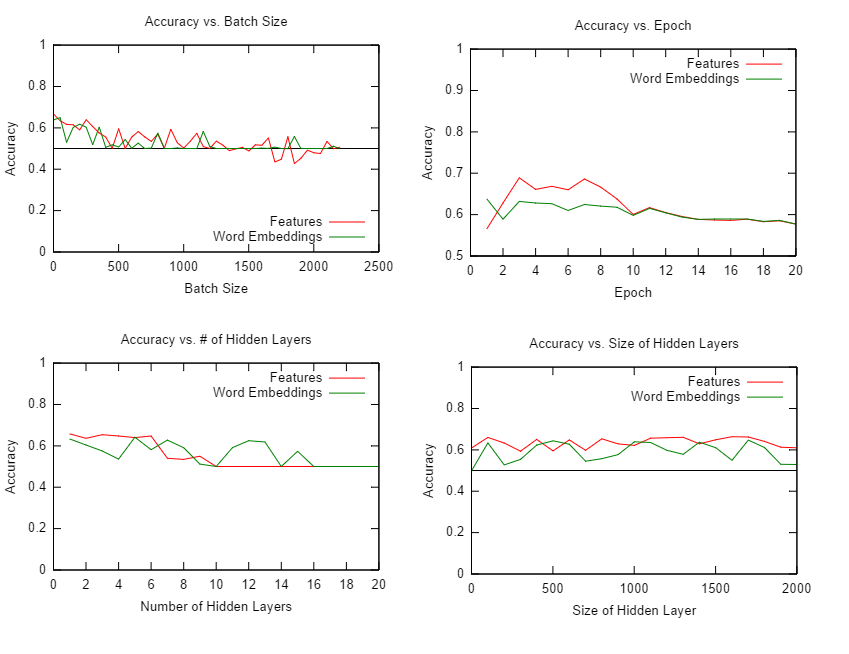
\includegraphics[width=1.2\linewidth]{images/all_in_one}
\caption{}
\label{fig:all_in_one}
\end{figure}

\subsubsection{Batch Sizes}
A Neural Network can be trained with batches of multiple training cases at a time. These batches (also known as minibatches) allow users to cut dataset into smaller segments, feed it through the Neural Network, and update the NN with the mean of the final gradient descent.
\par Having big batches allows the NN to learn from a big dataset faster, as the throughput of each operation is much higher. However, since the update is being done with the mean of the gradient descent of all the batch's training cases, it is possible to loose precision and over-fit to the training data.
\par Our experiments (Figure 1) clearly show that the NN performed better with batches of around 1 - 300 in size. Higher batches tended to converge to a 0.5 or worse accuracy, which could be attributed to overfitting. 


\subsubsection{\# of Hidden Layers}
- As we increase the number of hidden layers, our accuracy decreases. The reason for this is the gradient loss. (talk lots here)

\subsubsection{Size of Hidden Layers}
While increasing the size of a single hidden layer substantially decreased computational performance, it did not seem to affect the accuracy of the NN. However we did see a rise in dead-paths (i.e neural connections with weight = 0). It is important to mention however, that having a hidden layer that was smaller than the size of the input was actually detrimental to the performance while using Features as an input. This might be because the amount of neural paths are so limited that no real features can be distinguished. For the sake of performance, we that an apporpriate size for a layer was around 250-500.

\subsubsection{\# of Epochs}
The number of Epochs refers to the number of times an NN is trained with the same test data. Having multiple repetitions might be useful especially if you have a small training set, however too many repetitions can quickly lead to over-fitting. In our set of experiments we found that the optimum number of epochs was 2-3. Anything past this value, would slowly tend to overfit and thus produce worse results.

\subsection{Word Embeddings vs. Feature Vector}
The actual very best setup of Word Embeddings vs. Feature Vectore in Keras

\subsection{Keras vs. Our Own Neural Network}

\section{Further Work}

\subsection{Convolutional Networks}

\subsection{LSTM}

%References
%http://cs.ucsb.edu/~jod//papers/c-12-socialcom2013.pdf

\end{document}